\documentclass[aspectratio=169]{beamer}

\usepackage[T1]{fontenc} % Fixes the \textsc font substitution warning
\usepackage{amsmath}
\usepackage{amssymb}
\usepackage{graphicx}
\usepackage{tikz}
\usetikzlibrary{shapes.geometric, arrows.meta, positioning}

\definecolor{coolpurple}{HTML}{7f65a0}
\definecolor{lightpurple}{HTML}{ede8f5}
\definecolor{darktext}{HTML}{1a1a2e}
\definecolor{highlightpurple}{HTML}{5a3e82}

\setbeamercolor{normal text}{fg=darktext, bg=white}
\setbeamercolor{structure}{fg=coolpurple}
\setbeamercolor{frametitle}{fg=white, bg=coolpurple}
\setbeamercolor{title}{fg=white, bg=coolpurple}
\setbeamercolor{subtitle}{fg=white}
\setbeamercolor{date}{fg=coolpurple}
\setbeamercolor{author}{fg=coolpurple}
\setbeamercolor{item}{fg=coolpurple}
\setbeamercolor{subitem}{fg=coolpurple!70!black}
\setbeamercolor{block title}{bg=coolpurple, fg=white}
\setbeamercolor{block body}{bg=lightpurple, fg=darktext}
\setbeamercolor{alerted text}{fg=highlightpurple}

\setbeamertemplate{itemize item}{\color{coolpurple}$\blacktriangleright$}
\setbeamertemplate{itemize subitem}{\color{coolpurple!70}$\bullet$}
\setbeamertemplate{navigation symbols}{}
\setbeamertemplate{footline}{%
	\hfill\insertframenumber\,/\,\inserttotalframenumber\hspace{1em}\vspace{0.5em}
}

\newcommand{\hl}[1]{\textcolor{coolpurple}{\textbf{#1}}}
\newcommand{\R}{\mathbb{R}}

\title{EngageNet}
\subtitle{M2 Presentation - April 26, 2026}
\author{Lado Turmanidze, Luka Javakhishvili, Mariami Gadelia, Keso Chikhladze}
\institute{\small{Supervisors: Dr. Philipp M\"{u}ller \& Beso Mikaberidze}}
\date{April 26, 2026}

\begin{document}
	
	\begin{frame}
		\titlepage
	\end{frame}
	
	\begin{frame}{Today's Agenda}
		\begin{enumerate}
			\item \textbf{Refresher} - what we are doing and the BiMamba-TTA base architecture
			\item \textbf{Regression adaptation} - why Gaussian fails and our Beta distribution framework
			\item \textbf{TTA for regression} - Beta-based uncertainty, sample selection, and the test-time loss
			\item \textbf{Architectural contribution} - fixing the order-sensitivity of inter-modal fusion via Gumbel-Sinkhorn
		\end{enumerate}
	\end{frame}
	
	\begin{frame}{\textsc{Part 1:} Refresher - What We Are Doing}
		\begin{center}
			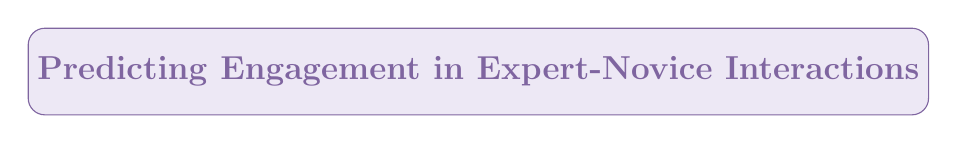
\begin{tikzpicture}
				\node[draw=coolpurple, fill=lightpurple, rounded corners=6pt,
				minimum width=9cm, minimum height=1.1cm, % Adjusted width to fix hbox
				font=\large\bfseries, text=coolpurple] {
					Predicting \textbf{Engagement} in Expert-Novice Interactions
				};
			\end{tikzpicture}
		\end{center}
		\begin{columns}[onlytextwidth]
			\begin{column}{0.6\textwidth}
				\begin{itemize}
					\item Inputs: video, audio, text, body pose, facial landmarks - all fused together.
					\item \textbf{Task:} predict a continuous score $y \in [0,1]$ frame-wise at **25 Hz**.
					\item Two corpora: \hl{NoXi} (Europe, FR/EN/DE) and \hl{NoXi+J} (Japan/China).
					\item Key challenge: \hl{cross-cultural domain shift} - train on NoXi, test on NoXi+J.
				\end{itemize}
			\end{column}
			\begin{column}{0.36\textwidth}
				\centering
				\scalebox{0.65}{
					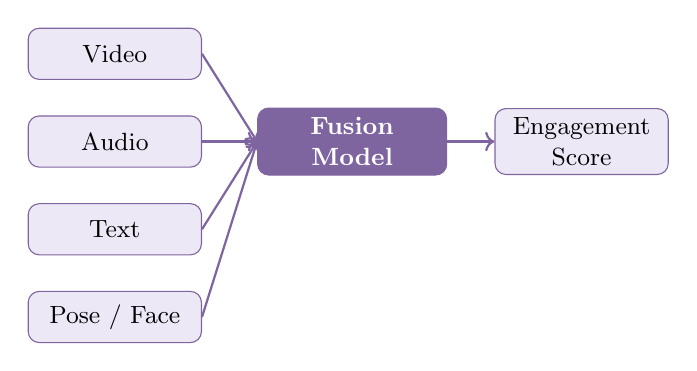
\begin{tikzpicture}[node distance=0.45cm, font=\small]
						\node[draw=coolpurple, fill=lightpurple, rounded corners, minimum width=2.2cm, minimum height=0.65cm, align=center] (video) {Video};
						\node[draw=coolpurple, fill=lightpurple, rounded corners, minimum width=2.2cm, minimum height=0.65cm, align=center, below=of video] (audio) {Audio};
						\node[draw=coolpurple, fill=lightpurple, rounded corners, minimum width=2.2cm, minimum height=0.65cm, align=center, below=of audio] (text) {Text};
						\node[draw=coolpurple, fill=lightpurple, rounded corners, minimum width=2.2cm, minimum height=0.65cm, align=center, below=of text] (pose) {Pose / Face};
						\node[draw=coolpurple, fill=coolpurple, rounded corners, minimum width=2.4cm, minimum height=0.85cm, align=center, right=0.7cm of audio, text=white, font=\small\bfseries] (model) {Fusion\\Model};
						\node[draw=coolpurple, fill=lightpurple, rounded corners, minimum width=2.2cm, minimum height=0.65cm, align=center, right=0.6cm of model] (out) {Engagement\\Score};
						\foreach \n in {video, audio, text, pose}
						\draw[->, thick, coolpurple] (\n.east) -- (model.west);
						\draw[->, thick, coolpurple] (model) -- (out);
					\end{tikzpicture}
				}
			\end{column}
		\end{columns}
	\end{frame}
	
	\begin{frame}{Refresher - BiMamba-TTA Architecture}
		\begin{columns}[onlytextwidth]
			\begin{column}{0.6\textwidth}
				Based on \textit{BiMamba-TTA} (Jia et al., NeurIPS 2025) - originally designed for emotion \textit{classification}.
				
				\vspace{0.5em}
				\textbf{Two modules:}
				\begin{enumerate}
					\item \hl{Intra-Modal BiMamba} - bidirectional SSM; captures temporal context.
					\item \hl{Inter-Modal BiMamba} - sweep \textit{across} modalities to share cross-stream information.
				\end{enumerate}
				\vspace{0.3em}
				A \textbf{TTA module} then adapts the model at test time using only the test samples themselves.
			\end{column}
			\begin{column}{0.40\textwidth}
				\centering
				\scalebox{0.85}{
					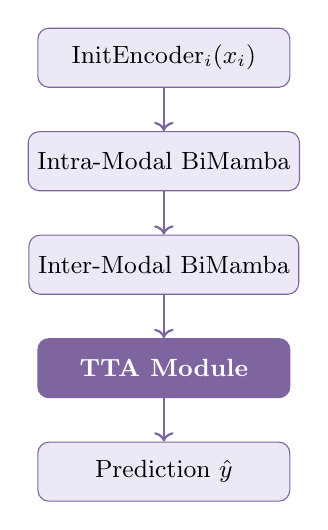
\begin{tikzpicture}[node distance=0.55cm, font=\small]
						\node[draw=coolpurple, fill=lightpurple, rounded corners, minimum width=3.2cm, minimum height=0.75cm, align=center] (enc) {InitEncoder$_i(x_i)$};
						\node[draw=coolpurple, fill=lightpurple, rounded corners, minimum width=3.2cm, minimum height=0.75cm, align=center, below=of enc] (intra) {Intra-Modal BiMamba};
						\node[draw=coolpurple, fill=lightpurple, rounded corners, minimum width=3.2cm, minimum height=0.75cm, align=center, below=of intra] (inter) {Inter-Modal BiMamba};
						\node[draw=coolpurple, fill=coolpurple, rounded corners, minimum width=3.2cm, minimum height=0.75cm, align=center, below=of inter, text=white, font=\small\bfseries] (tta) {TTA Module};
						\node[draw=coolpurple, fill=lightpurple, rounded corners, minimum width=3.2cm, minimum height=0.75cm, align=center, below=of tta] (out) {Prediction $\hat{y}$};
						\foreach \a/\b in {enc/intra, intra/inter, inter/tta, tta/out}
						\draw[->, thick, coolpurple] (\a) -- (\b);
					\end{tikzpicture}
				}
			\end{column}
		\end{columns}
	\end{frame}
	
	\begin{frame}{Refresher - Intra-Modal BiMamba}
		For each modality $i$, the encoder produces $h_i \in \R^{L' \times C_i'}$. The BiMamba block then:
		
		\vspace{0.3em}
		\begin{columns}[onlytextwidth]
			\begin{column}{0.50\textwidth}
				\begin{block}{(1) Gating}
					\small $g_i = \sigma(W_i^g h_i + b_i^g)$ \quad (SiLU) \\
					Highlights engagement-relevant features.
				\end{block}
				\begin{block}{(2) Bidirectional SSM scan}
					\small
					$h_i^{\rightarrow} = g_i \otimes \mathrm{SSM}_{\rightarrow}(\cdots)$ \\
					$h_i^{\leftarrow} = g_i \otimes \mathrm{SSM}_{\leftarrow}(\mathrm{Rev}_t(\cdots))$ \\
					$\otimes$ = Hadamard product.
				\end{block}
			\end{column}
			\begin{column}{0.46\textwidth}
				\begin{block}{(3) Residual output}
					\small
					$$ u_i = h_i + \left(W_i^o \frac{h_i^{\rightarrow} + \mathrm{Rev}_t(h_i^{\leftarrow})}{2} + b_i^o\right) $$
				\end{block}
				\vspace{0.3em}
				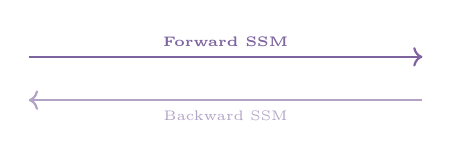
\begin{tikzpicture}
					\draw[->, thick, coolpurple] (-2.5,0) -- (2.5,0) node[midway, above, font=\tiny\bfseries] {Forward SSM};
					\draw[<-, thick, coolpurple!60] (-2.5,-0.55) -- (2.5,-0.55) node[midway, below, font=\tiny] {Backward SSM};
				\end{tikzpicture}
			\end{column}
		\end{columns}
	\end{frame}
	
	\begin{frame}{Refresher - Inter-Modal BiMamba \& TTA}
		\begin{columns}[onlytextwidth]
			\begin{column}{0.48\textwidth}
				\begin{block}{Inter-Modal BiMamba}
					\small
					Concatenate outputs and transpose:
					$$ m = (u_1 \circ \cdots \circ u_M)^\top \in \R^{(\sum C_i') \times L'} $$
					A second BiMamba sweeps across modalities.
				\end{block}
			\end{column}
			\begin{column}{0.48\textwidth}
				\begin{block}{Test-Time Adaptation}
					\small
					\textbf{Smart filter:} select samples that are confident overall but uncertain unimodally.
					
					\textbf{Surgical fine-tuning:} only update BatchNorm and the first layers. Core weights stay \hl{frozen}.
				\end{block}
			\end{column}
		\end{columns}
		\vspace{0.5em}
		\begin{center}
			
\begin{tikzpicture}
				\node[draw=coolpurple, fill=lightpurple, rounded corners=6pt,
				text width=0.95\textwidth, minimum height=1.0cm, align=center,
				font=\bfseries, text=coolpurple] {
					Everything above was originally designed for \textit{classification}. We adapt it to \textit{regression}.
				};
			\end{tikzpicture}
		\end{center}
	\end{frame}
	
	\begin{frame}{\textsc{Part 2:} Why Gaussian Fails for Engagement}
		\begin{columns}[onlytextwidth]
			\begin{column}{0.52\textwidth}
				$$ p(y \mid x) = \mathcal{N}(\hat{\mu}(x),\, \hat{\sigma}^2(x)) $$
				\begin{alertblock}{The problem}
					\small Engagement is \textbf{strictly bounded}: $y \in [0,1]$. \\
					A Gaussian assigns probability to $(-\infty, 0)$ and $(1, \infty)$ - \hl{probability leakage}. \\
					Poorly calibrated near boundaries.
				\end{alertblock}
			\end{column}
			\begin{column}{0.44\textwidth}
				\centering
				\scalebox{0.82}{
					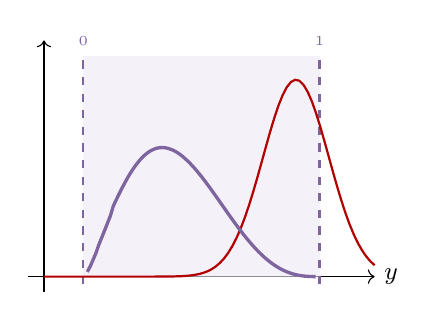
\begin{tikzpicture}[font=\small]
						\draw[->] (-0.2,0) -- (4.2,0) node[right] {$y$};
						\draw[->] (0,-0.2) -- (0,3.0);
						\fill[lightpurple, opacity=0.6] (0.5,0) rectangle (3.5,2.8);
						\draw[dashed, coolpurple, thick] (0.5,-0.1) -- (0.5,2.8) node[above, font=\tiny] {$0$};
						\draw[dashed, coolpurple, thick] (3.5,-0.1) -- (3.5,2.8) node[above, font=\tiny] {$1$};
						\draw[red!70!black, thick, domain=0:4.2, samples=80]
						plot(\x, {2.5*exp(-(\x-3.2)^2/0.35)});
						\draw[coolpurple, very thick, domain=0.55:3.45, samples=80]
						plot(\x, {2.3*(((\x-0.5)/3)^1.5)*((1-((\x-0.5)/3))^3)/0.08});
					\end{tikzpicture}
				}
			\end{column}
		\end{columns}
	\end{frame}
	
	\begin{frame}{The Beta Regression Framework}
		\small
		\begin{columns}[onlytextwidth]
			\begin{column}{0.48\textwidth}
				Support on $[0,1]$:
				$$ p(y \mid \alpha, \beta) = \frac{y^{\alpha-1}(1-y)^{\beta-1}}{B(\alpha,\beta)} $$
				Output shape parameters via softplus:
				$$ \alpha = \text{sp}(z_\alpha)+1, \quad \beta = \text{sp}(z_\beta)+1 $$
				Predictive mean:
				$$ \hat{\mu} = \frac{\alpha}{\alpha+\beta} $$
			\end{column}
			\begin{column}{0.48\textwidth}
				\begin{block}{Boundary-aware uncertainty}
					\footnotesize
					Variance naturally vanishes at boundaries:
					$$ \lim_{\hat{\mu}\to 0}\mathrm{Var}[y] = 0 $$
				\end{block}
				\begin{block}{Training loss}
					\footnotesize
					Beta negative log-likelihood:
					$$ \mathcal{L}_{\text{NLL}} = -(\hat{\alpha}-1)\ln y - (\hat{\beta}-1)\ln(1-y) + \ln B(\hat{\alpha},\hat{\beta}) $$
				\end{block}
			\end{column}
		\end{columns}
	\end{frame}
	
	\begin{frame}{TTA - Sample Selection \& Adaptive Thresholds}
		\begin{block}{Two-level filter}
			\centering\small
			\vspace{0.2em}
			$$ S(x) = \mathbb{I}\bigl\{\,U_{\text{multi}}(x) \leq \gamma_m(t) \;\text{ AND }\; \textstyle\sum w_i\, U_i(x) \geq \gamma_u(t)\,\bigr\} $$
			\vspace{0.2em}
		\end{block}
		
		\vspace{1em}
		\begin{block}{Uncertainty decomposition (MC Dropout)}
			\footnotesize
			$$ U_{\text{total}} = \underbrace{\frac{1}{T}\sum_t\mathrm{Var}[\text{Beta}_t]}_{\text{aleatoric}} + \underbrace{\frac{1}{T}\sum_t(\hat{\mu}^{(t)}-\bar{\mu})^2}_{\text{epistemic}} $$
			We \hl{adapt on high-epistemic samples}.
		\end{block}
	\end{frame}
	
	\begin{frame}{TTA - Test-Time Loss}
		\begin{block}{Mutual Information Sharing (MIS) loss}
			\footnotesize
			$$ \mathcal{L}_{\text{mis}} = \sum_{i=1}^M D_{KL}\!\bigl(\text{Beta}(\alpha_i,\beta_i)\;\|\;\text{Beta}(\alpha_{\text{multi}},\beta_{\text{multi}})\bigr) $$
			\begin{center}
				\resizebox{0.95\textwidth}{!}{% Use inline math inside resizebox to prevent display-math crash
					$\displaystyle D_{KL}(B_1\|B_2) = \ln\tfrac{B(\alpha_2,\beta_2)}{B(\alpha_1,\beta_1)} + (\alpha_1-\alpha_2)\psi(\alpha_1)+(\beta_1-\beta_2)\psi(\beta_1)+(\alpha_2-\alpha_1+\beta_2-\beta_1)\psi(\alpha_1+\beta_1)$
				}
			\end{center}
		\end{block}
		\begin{block}{Final TTA objective}
			\centering\small
			$$ \mathcal{L}_{\text{TTA}} = \mathcal{L}_{\text{mis}} + \lambda\displaystyle\sum_{i=1}^M \text{NLL}_{\text{Beta}}\!\bigl(\hat{\mu}_{\text{multi}},\,\alpha_i,\beta_i\bigr) $$
		\end{block}
	\end{frame}
	
	\begin{frame}{\textsc{Part 4:} The Order-Sensitivity Problem}
		\begin{center}
			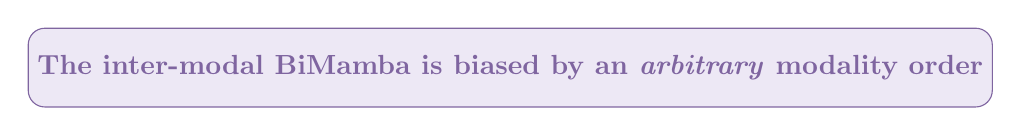
\begin{tikzpicture}
				\node[draw=coolpurple, fill=lightpurple, rounded corners=6pt,
				minimum width=10cm, minimum height=1.0cm,
				font=\bfseries, text=coolpurple] {
					The inter-modal BiMamba is biased by an \textit{arbitrary} modality order
				};
			\end{tikzpicture}
		\end{center}
		\begin{columns}[onlytextwidth]
			\begin{column}{0.5\textwidth}
				\small
				\textbf{Proposition.} For any SSM with $\bar{A} \neq I$, the output is \textbf{not permutation-invariant}. \\
				\textit{Sketch:} with $M=2$,
				$$ y_2 - y_2' = C\bar{B}(\bar{A}-I)(u_1 - u_2) \neq 0 $$
				Vanishes only if $\bar{A}=I$ (memoryless map).
			\end{column}
			\begin{column}{0.40\textwidth}
				\centering
				\scalebox{0.80}{
					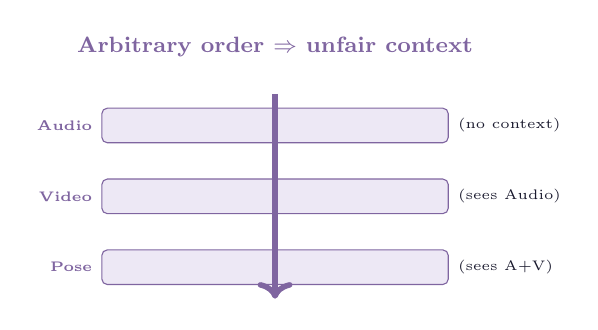
\begin{tikzpicture}[font=\small, node distance=0.3cm]
						\node[font=\bfseries\footnotesize, text=coolpurple] at (0, 2.6) {Arbitrary order $\Rightarrow$ unfair context};
						\foreach \y/\lbl/\ctx in {1.6/Audio/\text{(no context)}, 0.7/Video/\text{(sees Audio)}, -0.2/Pose/\text{(sees A+V)}} {
							\draw[fill=lightpurple, draw=coolpurple, rounded corners=2pt] (-2.2,\y-0.22) rectangle (2.2,\y+0.22);
							\node[left, text=coolpurple, font=\tiny\bfseries] at (-2.2,\y) {\lbl};
							\node[right, text=darktext, font=\tiny] at (2.2,\y) {$\ctx$};
						}
						\draw[->, line width=2pt, coolpurple] (0,2.0) -- (0,-0.6);
					\end{tikzpicture}
				}
			\end{column}
		\end{columns}
	\end{frame}
	
	\begin{frame}{Fix: Differentiable Modality Ordering via Gumbel-Sinkhorn}
		\begin{columns}[onlytextwidth]
			\begin{column}{0.54\textwidth}
				\footnotesize
				\textbf{(1) Score matrix.} Affinities:
				$$ Z_{ij} = \frac{q_i^\top k_j}{\sqrt{d_s}}, \quad q_i = W_Q\bar{u}_i,\; k_j = W_K\bar{u}_j $$
				\textbf{(2) Gumbel perturbation.} 
				$$ \tilde{Z}_{ij} = \frac{Z_{ij} + G_{ij}}{\tau} $$
			\end{column}
			\begin{column}{0.44\textwidth}
				\footnotesize
				\textbf{(3) Sinkhorn normalisation.} 
				$$ P = \text{Sinkhorn}(\exp(\tilde{Z})) $$
				\textbf{(4) Soft reordering.}
				$$ \tilde{u}_i = \sum_{j=1}^{M} P_{ij}\, u_j, \quad \tilde{m} = \text{Trans}(\tilde{u}_1 \circ \cdots \circ \tilde{u}_M) $$
			\end{column}
		\end{columns}
	\end{frame}
	
	\begin{frame}{Equivariance Guarantee \& Intuition}
		\begin{columns}[onlytextwidth]
			\begin{column}{0.52\textwidth}
				\begin{block}{Equivariance guarantee}
					\footnotesize Relabelling modalities by $\rho \in S_M$ transforms the permutation as $\pi^*_\rho = \rho \circ \pi^*$. Representation $H$ is \hl{invariant to concatenation order}.
				\end{block}
				\begin{block}{Connection to mHC}
					\footnotesize Uses the same Sinkhorn-Knopp machinery as our mHC residual idea.
				\end{block}
			\end{column}
			\begin{column}{0.44\textwidth}
				\centering
				\scalebox{0.72}{
					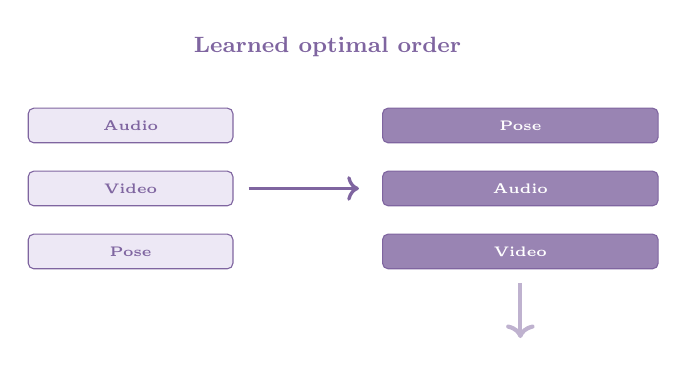
\begin{tikzpicture}[font=\small, node distance=0.45cm]
						\node[font=\bfseries\footnotesize, text=coolpurple] at (0, 3.4) {Learned optimal order};
						\foreach \y/\lbl in {2.4/Audio, 1.6/Video, 0.8/Pose} {
							\draw[fill=lightpurple, draw=coolpurple, rounded corners=2pt] (-3.8,\y-0.22) rectangle (-1.2,\y+0.22);
							\node[text=coolpurple, font=\tiny\bfseries] at (-2.5,\y) {\lbl};
						}
						\draw[->, very thick, coolpurple] (-1.0, 1.6) -- (0.4, 1.6);
						\foreach \y/\lbl in {2.4/Pose, 1.6/Audio, 0.8/Video} {
							\draw[fill=coolpurple!80, draw=coolpurple, rounded corners=2pt] (0.7,\y-0.22) rectangle (4.2,\y+0.22);
							\node[text=white, font=\tiny\bfseries] at (2.45,\y) {\lbl};
						}
						\draw[->, line width=1.5pt, coolpurple!50] (2.45, 0.4) -- (2.45,-0.3);
					\end{tikzpicture}
				}
			\end{column}
		\end{columns}
	\end{frame}
	
	\begin{frame}{Summary \& Next Steps}
		\begin{columns}[onlytextwidth]
			\begin{column}{0.31\textwidth}
				\begin{block}{What we formalised}
					\small Beta head, variance-as-entropy proxy, and surgical fine-tuning.
				\end{block}
			\end{column}
			\begin{column}{0.31\textwidth}
				\begin{block}{Novel architectural contribution}
					\small Permutation-equivariant inter-modal fusion via Gumbel-Sinkhorn.
				\end{block}
			\end{column}
			\begin{column}{0.31\textwidth}
				\begin{block}{Next steps}
					\small Evaluate NoXi $\to$ NoXi+J with/without TTA.
				\end{block}
			\end{column}
		\end{columns}
		\vspace{1em}
		\begin{center}
			\Large\bfseries\color{coolpurple} Time to implement!
		\end{center}
	\end{frame}
	
\end{document}